%%% DOCUMENTCLASS 
%%%-------------------------------------------------------------------------------

\documentclass[a4paper,11pt, onecolumn, openany]{memoir}

%%% PACKAGES 
%%%------------------------------------------------------------------------------

\usepackage[utf8]{inputenc} % If utf8 encoding
% \usepackage[lantin1]{inputenc} % If not utf8 encoding, then this is probably the way to go
\usepackage[T1]{fontenc}
\usepackage{polski}
\usepackage[polish]{babel} 
\usepackage[final]{microtype} % Less badboxes
\usepackage{tcolorbox}
\usepackage{natbib}
% \usepackage{kpfonts} %Font
\usepackage{lmodern}
\usepackage{tgpagella}
% \usepackage{tikz} % Figures
\usepackage{graphicx} % Include figures
\usepackage{import}
\graphicspath{ {ilustracje/} }
\definecolor{titlepagecolor}{cmyk}{0.7,.30,0,.40}
\definecolor{miejscekolor}{cmyk}{0,0,1,.10}
\definecolor{code-gray}{gray}{0.95} 
%%% PAGE LAYOUT 
%%%------------------------------------------------------------------------------

\setlrmarginsandblock{0.15\paperwidth}{*}{1} % Left and right margin
\setulmarginsandblock{0.2\paperwidth}{*}{1}  % Upper and lower margin
\checkandfixthelayout


%%% INTERNAL HYPERLINKS
%%%-------------------------------------------------------------------------------

\usepackage{hyperref}   % Internal hyperlinks
\hypersetup{
	pdfborder={0 0 0},      % No borders around internal hyperlinks
	pdfauthor={Tomasz Nycz} % author
}
\usepackage{memhfixc}   %

%%% THE DOCUMENT
%%% Where all the important stuff is included!
%%%-------------------------------------------------------------------------------

\author{Tomasz Nycz}
\title{Formaty i relacje przestrzenne w QGIS}

\usepackage{lipsum} % Just to put in some text

\begin{document}
	
	\frontmatter
	
	\maketitle
	
	\begin{abstract}
		Robię co mogę
	\end{abstract}
	\clearpage
	
	\tableofcontents*
	\clearpage

\part{Odniesienia przestrzenne}
	\chapter{Zbiory danych przestrzennych}
		\section{Wymagania prawne}
			\subsection{GML}
		\section{GeoPackage - następca Shapefile}
			\subsection{Tworzenie zbioru Geopackage}
			\subsection{Połączenie ze zbiorem}
		\section{Baza danych w GeoPackage}
			\subsection{Dodawanie wielu warstw}
			\subsection{Dołączanie projektu}
			\subsection{Dołączanie symboli i styli}		

	\chapter{Układy współrzędnych}
		\section{CRS i układ współrzędnych}
		W środowisku GIS możemy spotkać się z pojęciami CRS, odwzorowania kartograficznego, układu współrzędnych, oraz tzw. datum czy gridshift. Do dalszej komfortowej pracy konieczne jest zapoznanie się z nimi, oraz ich wzajemnymi powiązaniami.
	
		\section{Uwarunkowania prawne}
		Wymagania prawne co do stosowanych układów odniesienia zdefiniowane są w rozporządzeniu Rady Ministrów z dnia 15 października 2012 r. w sprawie państwowego systemu odniesień przestrzennych (Dz.U. 2012 poz. 1247)\footnote{http://isap.sejm.gov.pl/isap.nsf/DocDetails.xsp?id=WDU20120001247}.
\begin{tcolorbox}[colback=black!5!white,colframe=white!55!black,title=§ 15. 1 i 2 rozporządzenia]
	§ 15. 1. Państwowy system odniesień przestrzennych stosuje się w pracach geodezyjnych i kartograficznych oraz przy
tworzeniu zbiorów danych przestrzennych przez organy władzy publicznej, przy czym:
\begin{enumerate}
	\item układ współrzędnych PL-LAEA stosuje się na potrzeby analiz przestrzennych i sprawozdawczości na poziomie ogólnoeuropejskim;
	\item układ współrzędnych PL-LCC stosuje się na potrzeby wydawania map w skali 1:500 000 i w mniejszych skalach;
	\item układ współrzędnych PL-UTM stosuje się na potrzeby wydawania standardowych opracowań kartograficznych w skalach od 1:10 000 do 1:250 000, wydawania map morskich oraz wydawania innych map przeznaczonych na potrzeby
	bezpieczeństwa i obronności państwa;
	\item układ współrzędnych PL-2000 stosuje się na potrzeby wykonywania map w skalach większych od 1:10 000 – w szczególności mapy ewidencyjnej i mapy zasadniczej.
\end{enumerate}
2. W pracach geodezyjnych i kartograficznych innych niż wymienione w ust. 1 pkt 1–4 stosuje się układ współrzędnych
PL-UTM lub układ współrzędnych PL-1992.
\end{tcolorbox}	
			\subsection{PUWG 92}
			\subsection{PUWG 2000}
			\subsection{UTM i LAEA}
		\section{Starsze układy współrzędnych}
		\section{Ćwiczenia}
		\subsection{Przypisanie CRS warstwy rastrowej}
		W tym ćwiczeniu wykorzystamy zbiory numerycznego modelu terenu w formacie ASCII GRID (.asc) udostępniane poprzez Główny Urząd Geodezji i Kartografii. 
		W katalogu "/modul1/crs/dtm" znajdziemy przykładowe pliki w takim formacie. Otwieramy okno \textbf{Data Source Manager}, z paska narzędzi lub przy pomocy skrótu (Ctrl+L) i wskazujemy w zakładce przeglądarka nasz plik rastrowy z dysku. 
		Zwróć uwagę na ikonkę \emph{znaku zapytania} znajdującą się po prawej stronie nazwy warstwy wyświetlanej na liście.
		\begin{figure}[!ht]
			\centering
			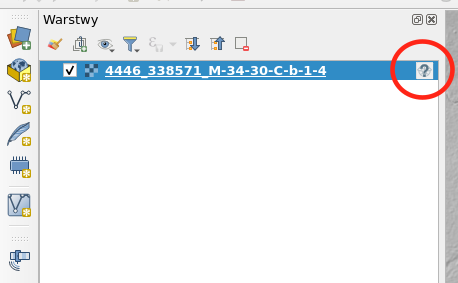
\includegraphics[width=10cm]{crs-cwiczenie1-brak-crs}
			\caption{Ostrzeżenie o braku zdefiniowanego CRS}
		\end{figure} 
	Po najechaniu na ten symbol i kliknięciu otworzy się nam okno \textbf{Wybór układu współrzędnych}. W polu filtra możemy szybko odszukać potrzebny nam układ - w tym wypadku \emph{ETRS89 / Poland CS92} o kodzie EPSG:2180. Po zatwierdzeniu \emph{OK} wracamy do głównego okna mapy.
	\begin{figure}[!ht]
    	\centering
	    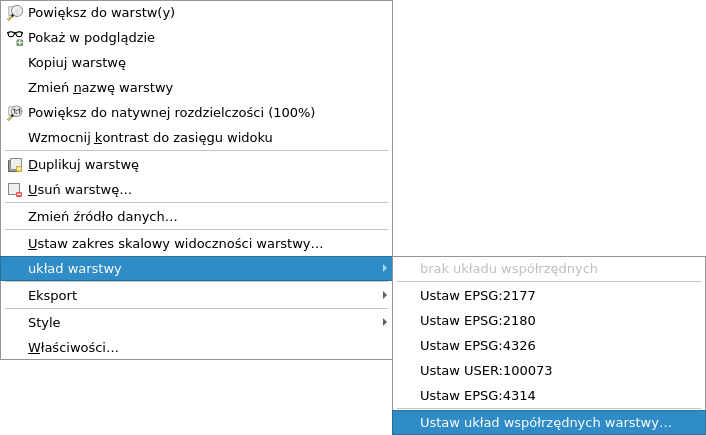
\includegraphics[width=10cm]{crs-cwiczenie1-menu-kontekstowe}
    	\caption{Menu kontekstowe warstwy - Ustawienie CRS}
    \end{figure} 
		\subsection{Zmiana odwzorowania rastra}
		W kolejnym ćwiczeniu zmienimy odwzorowanie naszej warstwy rastrowej i zapiszemy nowy zbiór na dysku.
		Wykorzystamy uprzednio otwarty raster NMT. Nasze zadanie możemy wykonać na dwa sposoby. Pierwszym jest wykorzystanie algorytmu processingu \textbf{Zmień odwzorowanie}. Ukaże się nam okno algorytmu, w którym wskazujemy kolejno:
		\begin{enumerate}
			\item warstwę wejściową
			\item źródłowy układ współrzędnych
			\item docelowy układ współrzędnych
			\item metodę resamplingu
			\item możliwe jest zdefiniowanie wartości NODATA
			\item dodatkowe parametry GDAL (np. kafelkowanie, typ kompresji)
			\item czy warstwa wyjściowa ma być zapisana na dysk, czy tylko wyświetlona jako tymczasowa
		\end{enumerate}
		\begin{figure}[!ht]
		\centering
		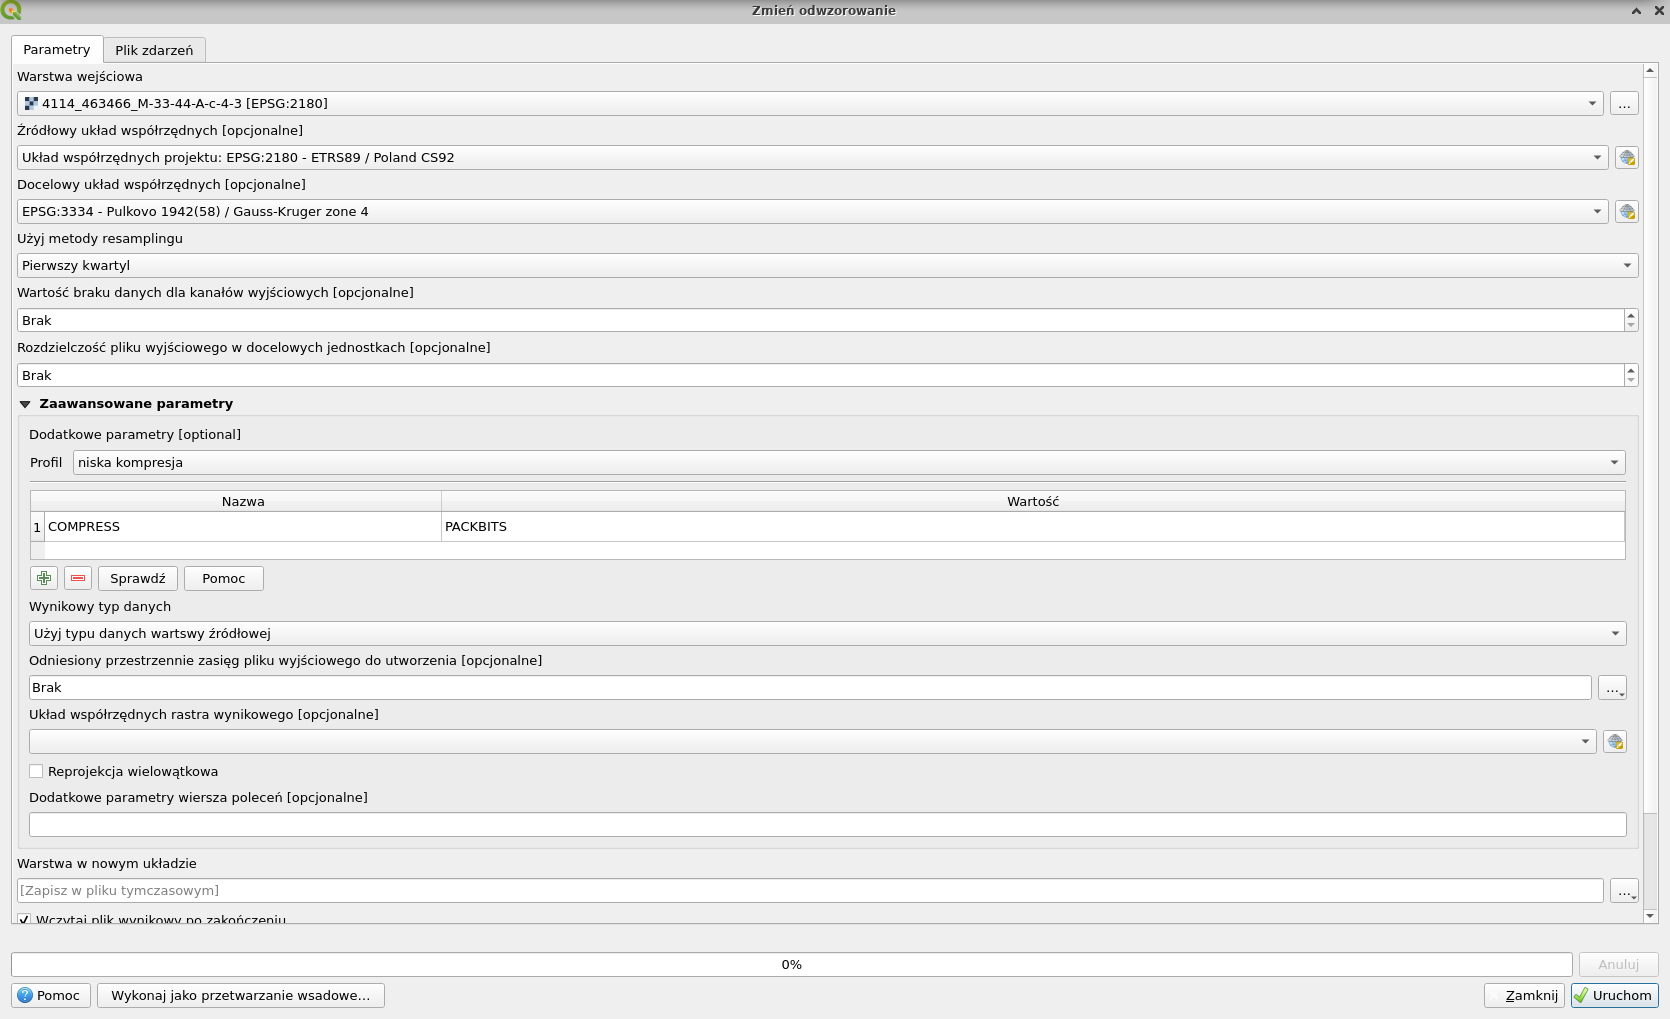
\includegraphics[width=10cm]{crs-cwiczenie2-zmien}
		\caption{Zmiana odwzorowania rastra}
	\end{figure} 
		Po zatwierdzeniu następuje transformacja rastra, która zależnie od jego wielkości może potrwać nawet kilkadziesiąt sekund.
		Druga metodą polega na zapisaniu istniejącej warstwy przy pomocy menu kontekstowego Eksport -> Zapisz Jako.
	\begin{figure}[!ht]
	\centering
	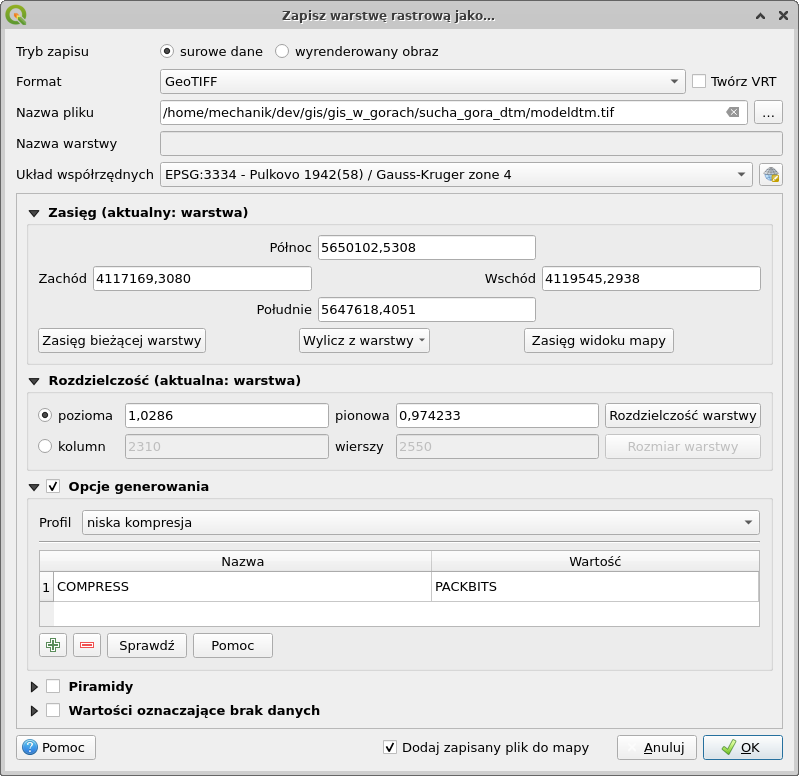
\includegraphics[width=10cm]{crs-cwiczenie2-zapisz-raster}
	\caption{Menu kontekstowe warstwy - Eksport Zapisz Jako}
\end{figure} 		
W tym wypadku również wskazujemy docelowy układ współrzędnych, ale również możemy wygodnie wskazać docelową rozdzielczość rastra.
	\chapter{Praca z archiwalnymi rastrami}
		\section{Wprowadzenie}
		\section{Referencja do punktów wspólnych}
		\section{Referencja do narożników mapy}
		\section{Ćwiczenia}

	\chapter{Referencja liniowa}
		\section{Wprowadzenie}
		\section{Przygotowanie zbioru liniowego}
		\section{Wyszukiwanie lokalizacji}
		\section{Ćwiczenia}

\part{Analiza}
	\chapter{Numeryczny model terenu - wprowadzenie}
		\section{Mapa spadków}
		\section{Mapa ekspozycji}
		\section{Inne wskaźniki topograficzne}
		\section{Ćwiczenia}
			\subsection{Wyznaczenie strefy narażonej osuwiskowo}
			\subsection{Stok narciarski}
	Wyszukanie stoku o ekspozycji północnej oraz nachylonego 10-30 stopni, wykorzystanie fuzzy logic
	\chapter{Widocznosc obiektów}
\section{Dominanty krajobrazu}
\section{Osie widokowe}
\section{Ćwiczenia}

\chapter{Nasłonecznienie}
\section{Mapa nasłonecznienia}
\section{Zmiana warunków}
\section{Potencjał solarny}
\section{Ćwiczenia}
\subsection{Strefy cienia}
\subsection{Jakość powierzchni dachowych dla fotowoltaiki}

\chapter{Wskaźniki urbanizacyjne}
\section{Powierzchnia zabudowy}
\section{Wskaźnik intensywności zabudowy}
\section{Powierzchnia biologicznie czynna}
\section{Ćwiczenia}
\subsection{Wyliczanie powierzchni zabudowy}

\chapter{Publikacja w internecie}
\section{GeoPDF}
\section{Strona html z osadzoną mapą}
\section{Geoportal Lizmap/QWC}
\section{Usługi w chmurze}
\section{Ćwiczenia}
\subsection{Nowa droga rowerowa}
\subsection{Plan zagospodarowania} 
\backmatter	
%%% BIBLIOGRAPHY
%%% -------------------------------------------------------------

% \bibliographystyle{utphysics}
% \bibliography{ref}

\end{document}